\newpage

\section{Histograms and Normal Distribution of Photocell Readings}
\label{s:photocell}

\subsection{Parts List}

\begin{enumerate}[itemsep=-5pt]
\item Laptop
\item CPX/CPB
\item USB Cable
\item Photocell
\item Resistor (10 kOhm)
\item Alligator Clips (x3)
\item Breadboard
\end{enumerate}

\subsection{Learning Objectives}
\begin{enumerate}[itemsep=-5pt]
\item Understand how a photocell responds to light level by measuring the voltage across the photocell in different light conditions
\item Learn how to create histograms of a noisy data signal
\item Understand mean and standard deviation and how that applies to Normal distributions.
\end{enumerate}

\subsection{Getting Started}

This lab is going to be similar to the potentiometer lab (See chapter \ref{s:voltage}). We are going to use a photocell though to vary the resistance instead of a potentiometer. A photocell (or Light Dependent Resistor, LDR) is a sensor whose resistance changes significantly based on the intensity of light falling on its sensitive surface. In dimmer light, its resistance is high, and in brighter light, its resistance is low. By integrating it into a simple voltage divider circuit similar to what you did for the potentiometer lab, you'll be able to read the voltage across the photocell and correlate that to light level. 

Wiring a photocell is similar to a potentiometer and remember that you need a resistor in series with the photocell to create the voltage divider circuit. There is a relevant \href{https://learn.adafruit.com/photocells/circuitpython}{Adafruit Tutorial on Photocells} and the code required to measure the voltage if you’d like to read more about it. The lab this week requires you to do the same as the potentiometer lab. I’d like you to wire up the circuit, take data at the low and high value of the photocell by covering the sensor with your finger and then shining a light on it and plotting the entire data set in Python on your desktop computer. A photo of the circuit is shown below. An alligator clip is connected to 3.3V on the CPX and the other end is connected to either end of the photocell. The photocell is then in series with a resistor and the other end of the resistor is connected to GND via another alligator clip. Finally, take another alligator clip from pin A2 and plug it into the same row on the breadboard as the resistor and photocell. Building this circuit as a voltage divider will create the standard voltage divider law given by the equation below.
\begin{equation}
V_{photocell} = V_{out}\frac{R_{photocell}}{R_{series}+R_{photocell}}
\end{equation}
In this case $V_{out}$ is 3.3V and $R_{series}$ is dependant on the resistor you use in your circuit. So, if you measure $V_{photocell}$ using the ADC on the CPX/CPB you'll be able to solve for the resistance in the photocell $R_{photocell}$. The resistance can then be used to determine the lux value. Some \href{https://www.researchgate.net/publication/375038565_Measuring_the_Voltage_Current_and_Resistance_of_the_LDR_Sensor_through_the_Arduino_UNO}{sources} suggest that Lux is a power law given by the equation below \cite{photocell2023}.
\begin{equation}
Lux = 500000R_{photocell}^{-0.7}
\end{equation}
where $R_{photocell}$ is the resistance of the photocell in Ohms.
\begin{figure}[H]
  \begin{center}
    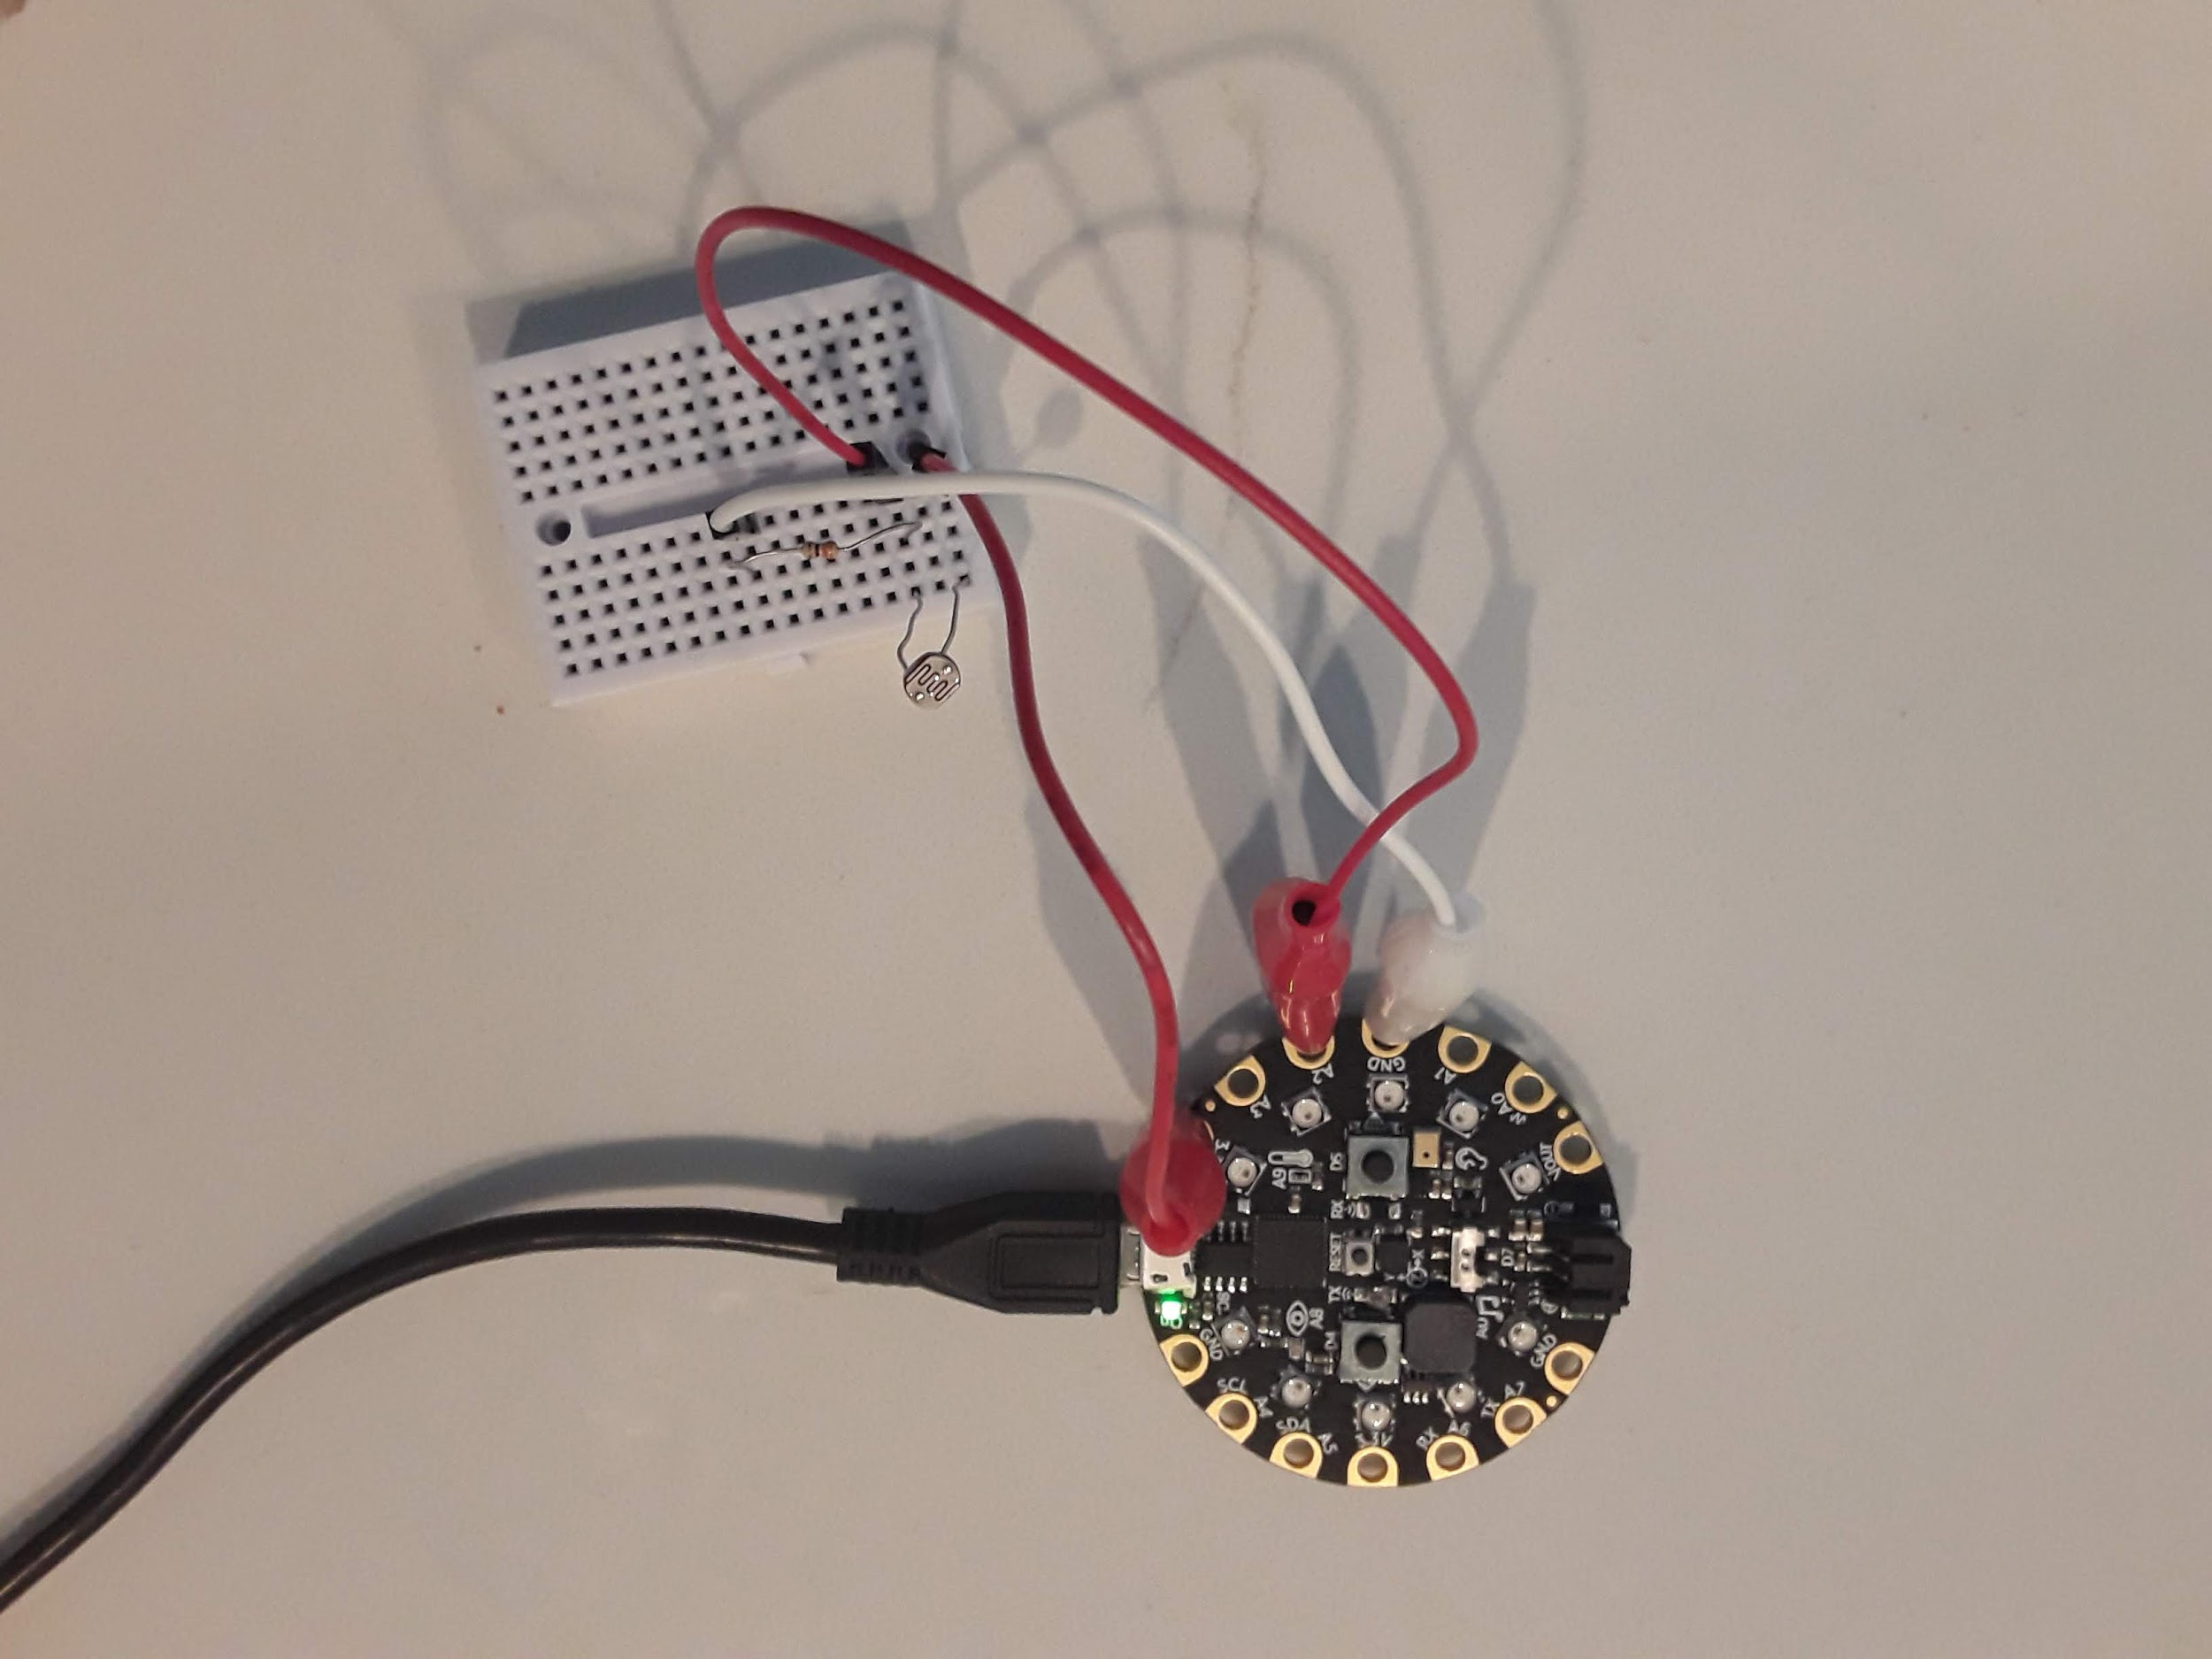
\includegraphics[width=\textwidth]{Figures/photocell_circuit.jpeg}
  \end{center}
\end{figure}
Once you have the
circuit wired properly you can use
the \href{https://github.com/cmontalvo251/Microcontrollers/blob/master/Circuit_Playground/CircuitPython/Analog/analog_simple.py}{same
code as the potentiometer lab}. The example screenshot below shows the
analog signal below showing a high spike where I placed a flashlight
over the photocell and then a low spot where I covered the photocell
with my finger. Remember that you can use any Analog pin on the CPX
provided you change line 5 to the same pin. 

\begin{figure}[H]
  \begin{center}
    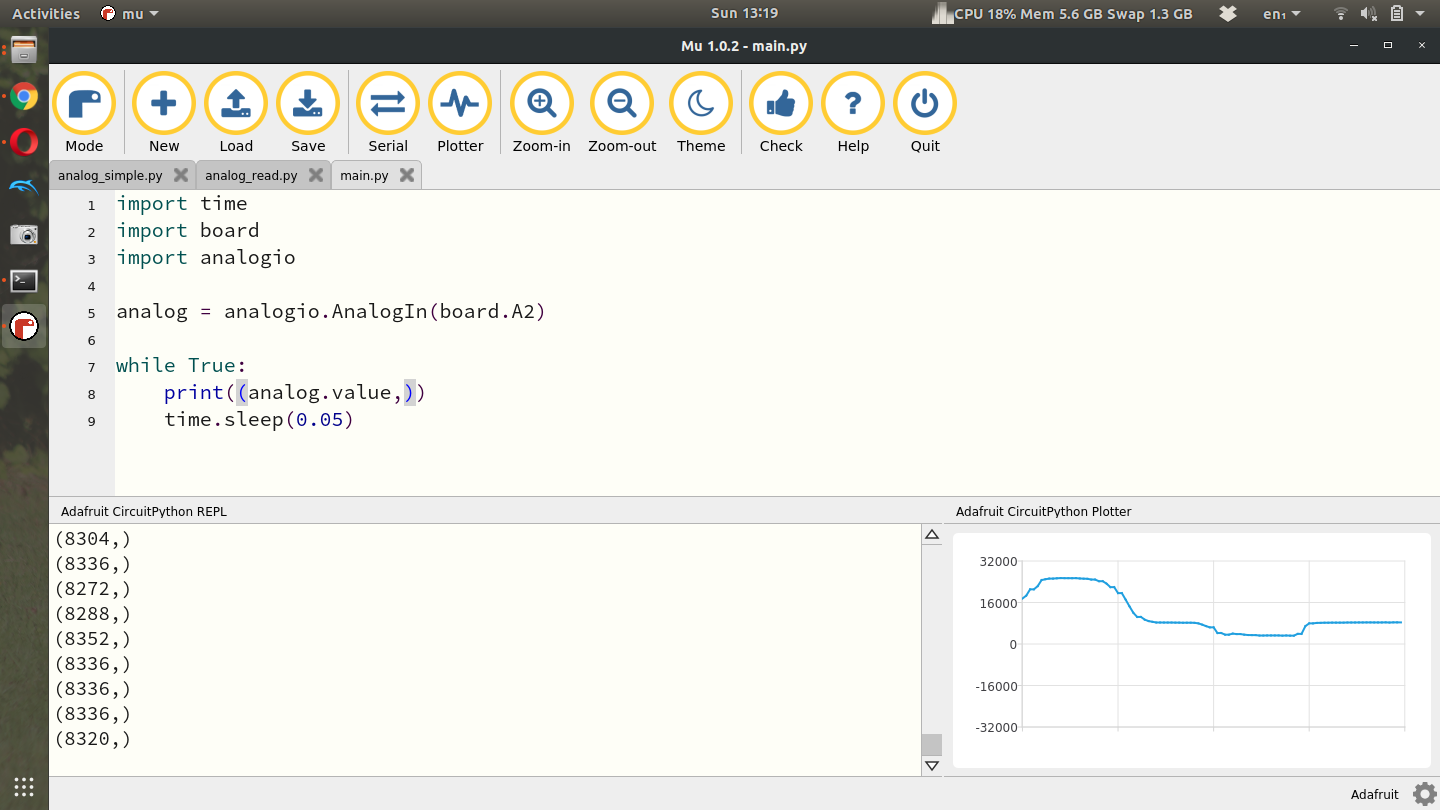
\includegraphics[width=\textwidth]{Figures/photocell_mu.png}
  \end{center}
\end{figure}
Once you’ve gotten some example data you can plot the result in Python as you did for the potentiometer lab. Here’s what your plot may look like.
\begin{figure}[H]
  \begin{center}
    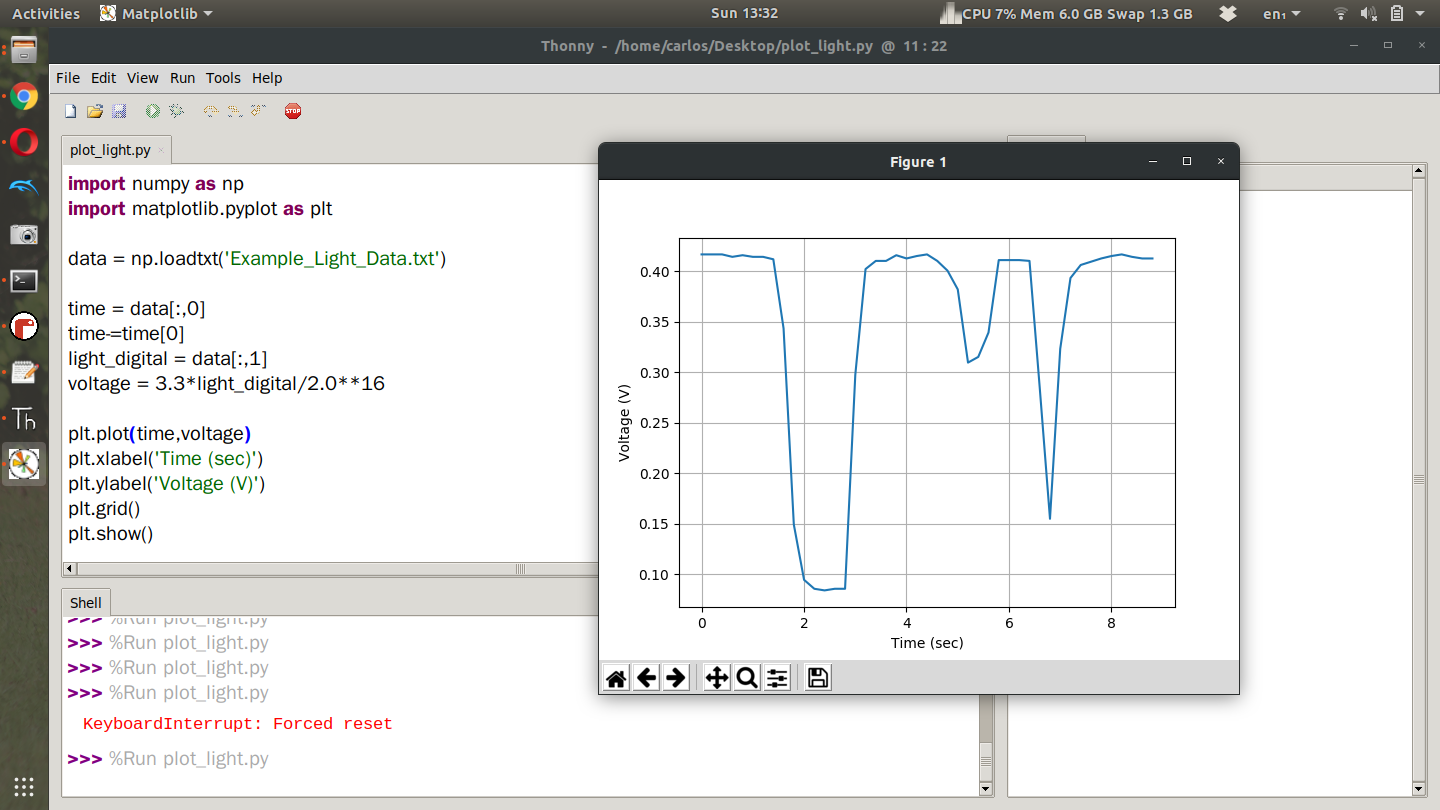
\includegraphics[width=\textwidth]{Figures/photocell_plots.png}
  \end{center}
\end{figure}
If you noticed the data you obtained even when the light source was
constant was quite noisy. What I’d like you to do for part 2 of this
lab is take 100 data points with the photocell with as constant of a
light source as possible. Do this for three different light
ranges. Low Light, ambient light and then sunlight if you're
outside. If you're completing this assignment late you can use a
flashlight as your third light source. With the three
different data streams, create a histogram of the data with
appropriate labels and compute the mean, median, and standard
deviation of the data
stream. \href{https://www.youtube.com/watch?v=bfeJfAWTqzY&list=PL_D7_GvGz-v1RsDs_OdNW65qRjEjmpfQx&index=22&t=0s}{Creating
a histogram in Python is fairly simple and I have a Youtube Video} to
supplement this tutorial. I also have another video where I
get \href{https://www.youtube.com/watch?v=e4xs9Ky7_YI&list=PL_D7_GvGz-v1RsDs_OdNW65qRjEjmpfQx&index=20&t=0s}{mean
and median values for accelerometer data}. Still, here is my example
code showing code to get mean, median, and standard deviation as well
as create the histogram. Notice in my code I imported the statistics
module to compute the mode. Although it worked in my code, it’s not
typical to compute the mode of a continuous variable because often
times you will not ever get the same value twice. Still, feel free to
compute the mode if you so desire. 
\begin{figure}[H]
  \begin{center}
    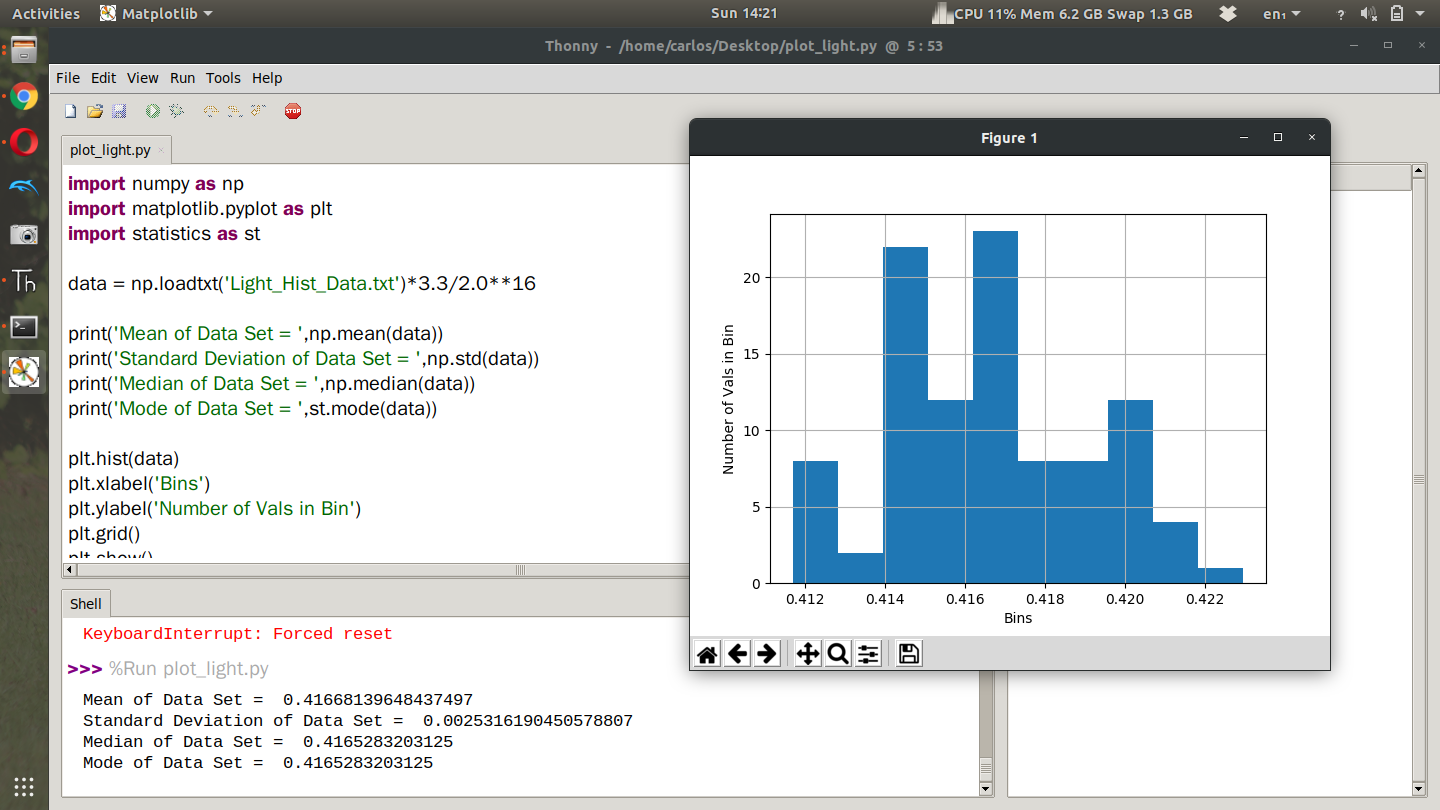
\includegraphics[width=\textwidth]{Figures/histogram.png}
  \end{center}
\end{figure}
Again make sure to convert to voltage before you plot that way you can see what the noise level is in volts. Notice that I import the data and convert to voltage all in one line. However, note that my text file only has 1 column of data. It’s possible your data has time in the first column and light value in the second column at which point you will need to extract the second column first and then convert to voltage. If you have two columns of data you’ll need to add a few things. First, don’t convert to voltage when you import the data.
\begin{verbatim}
data = np.loadtxt(‘Light_Hist_Data.txt’)
\end{verbatim}
Then extract the second column (assuming your photocell readings are in that column)
\begin{verbatim}
second_column = data[:,1]
\end{verbatim}
Finally convert to voltage
\begin{verbatim}
voltage = second_column*3.3/2.0**16
\end{verbatim}
Then replace data in the rest of your code with voltage. Remember to remove st.mode since it does not work all ofthe time for continuous data sets. 
\subsection{Throwing Out Outliers}
When I ran this experiment for a second time my CPX started and stopped 3 separate times. You'll see in the time series plot below that the voltage dipped in the first set and the second data set had some weird bumps probably from me changing tabs on my chrome tab. The photocell was close to my computer so that effected it. Thankfully the 3rd data set looked pretty good.
\begin{figure}[H]
  \begin{center}
    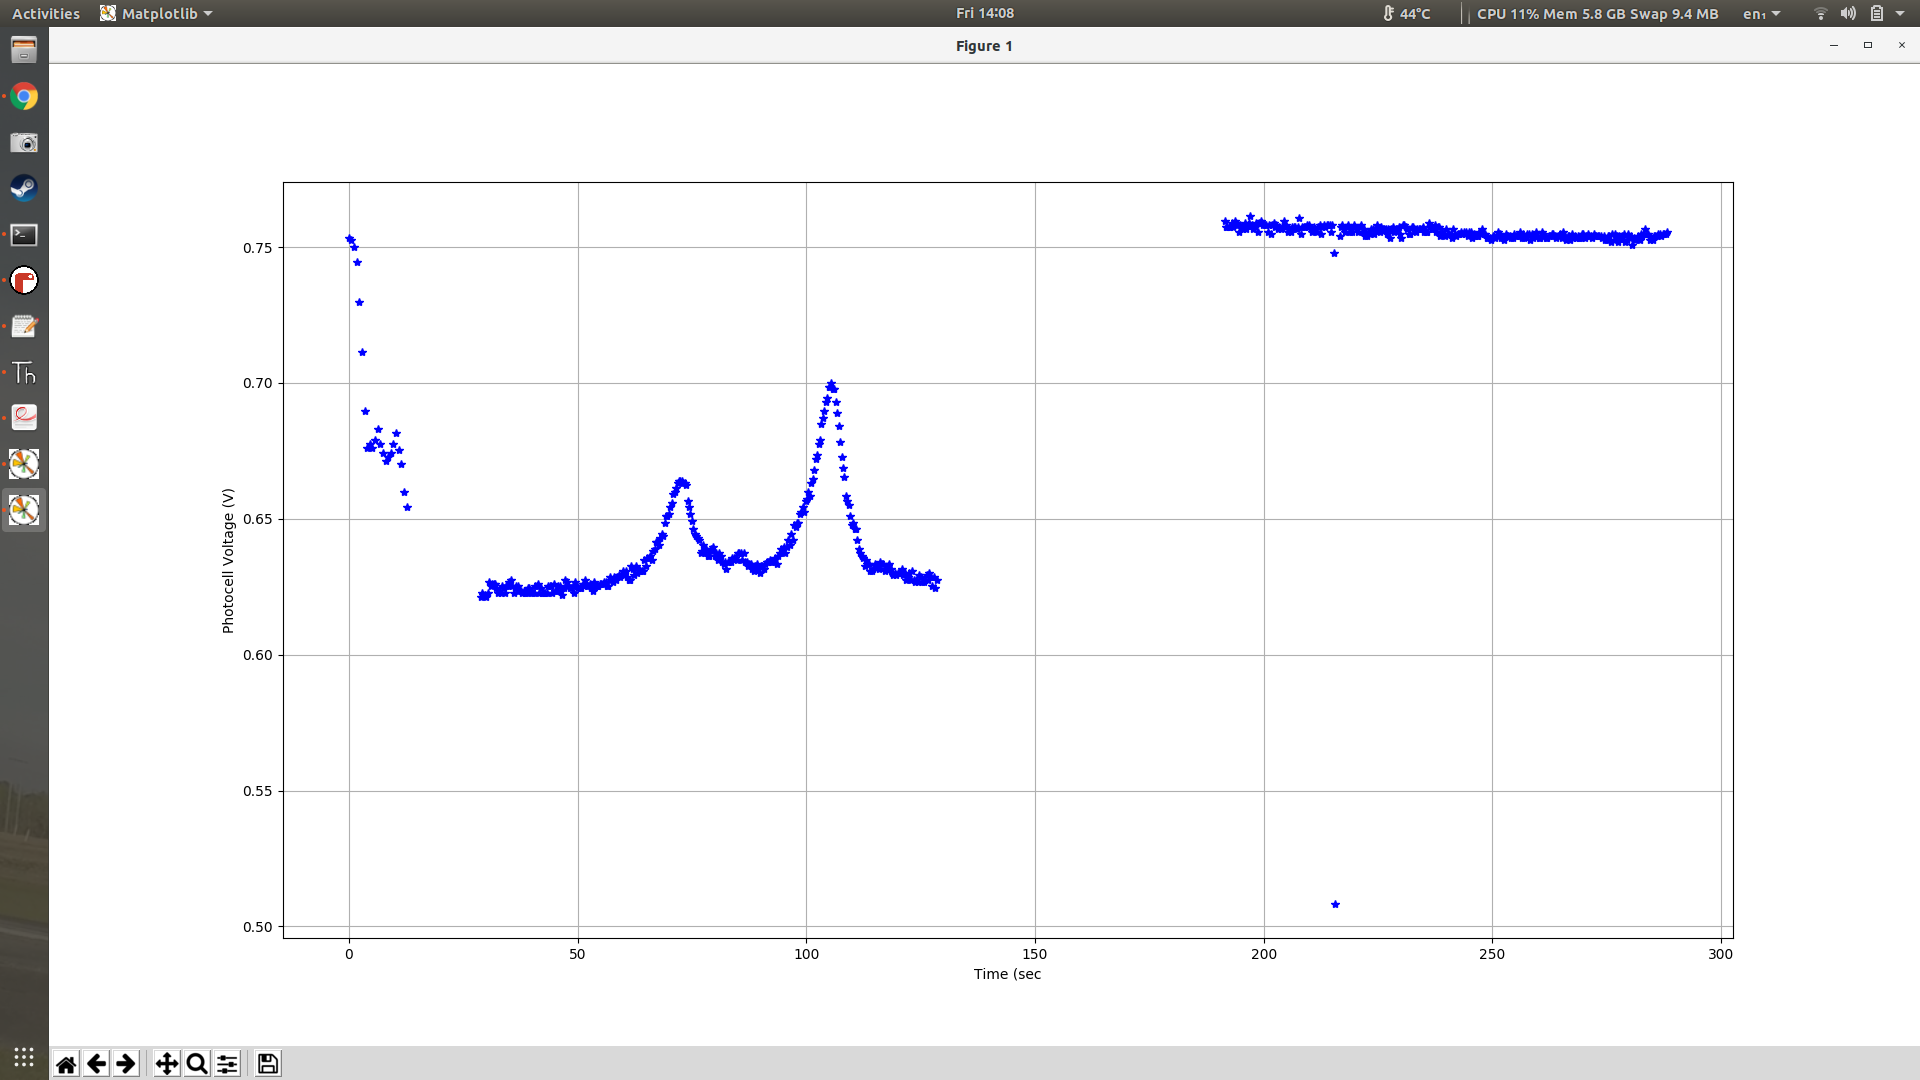
\includegraphics[width=\textwidth]{Figures/photocell_bad.png}
  \end{center}
\end{figure}
The only problem with the 3rd data set is that I put my hand over it for testing purposes. Because of that I had to remove those outliers. To do that I computed the current mean and standard deviation and then threw out all data points that were 3 standard deviations away from the mean. The code looks like this.
\begin{verbatim}
##COMPUTE CURRENT MEAN AND DEV 

mean = np.mean(voltage) 

dev = np.std(voltage) 

print(mean,dev) 

time = time[voltage > mean - 3*dev]

voltage = voltage[voltage > mean - 3*dev] 

time = time[voltage < mean + 3*dev] 

voltage = voltage[voltage < mean + 3*dev]

###COMPUTE NEW MEAN,STD 

mean = np.mean(voltage) 

dev = np.std(voltage) print(mean,dev)
\end{verbatim}

Once I did all that clean up I was able to get a nice time series plot of my data. 
\begin{figure}[H]
  \begin{center}
    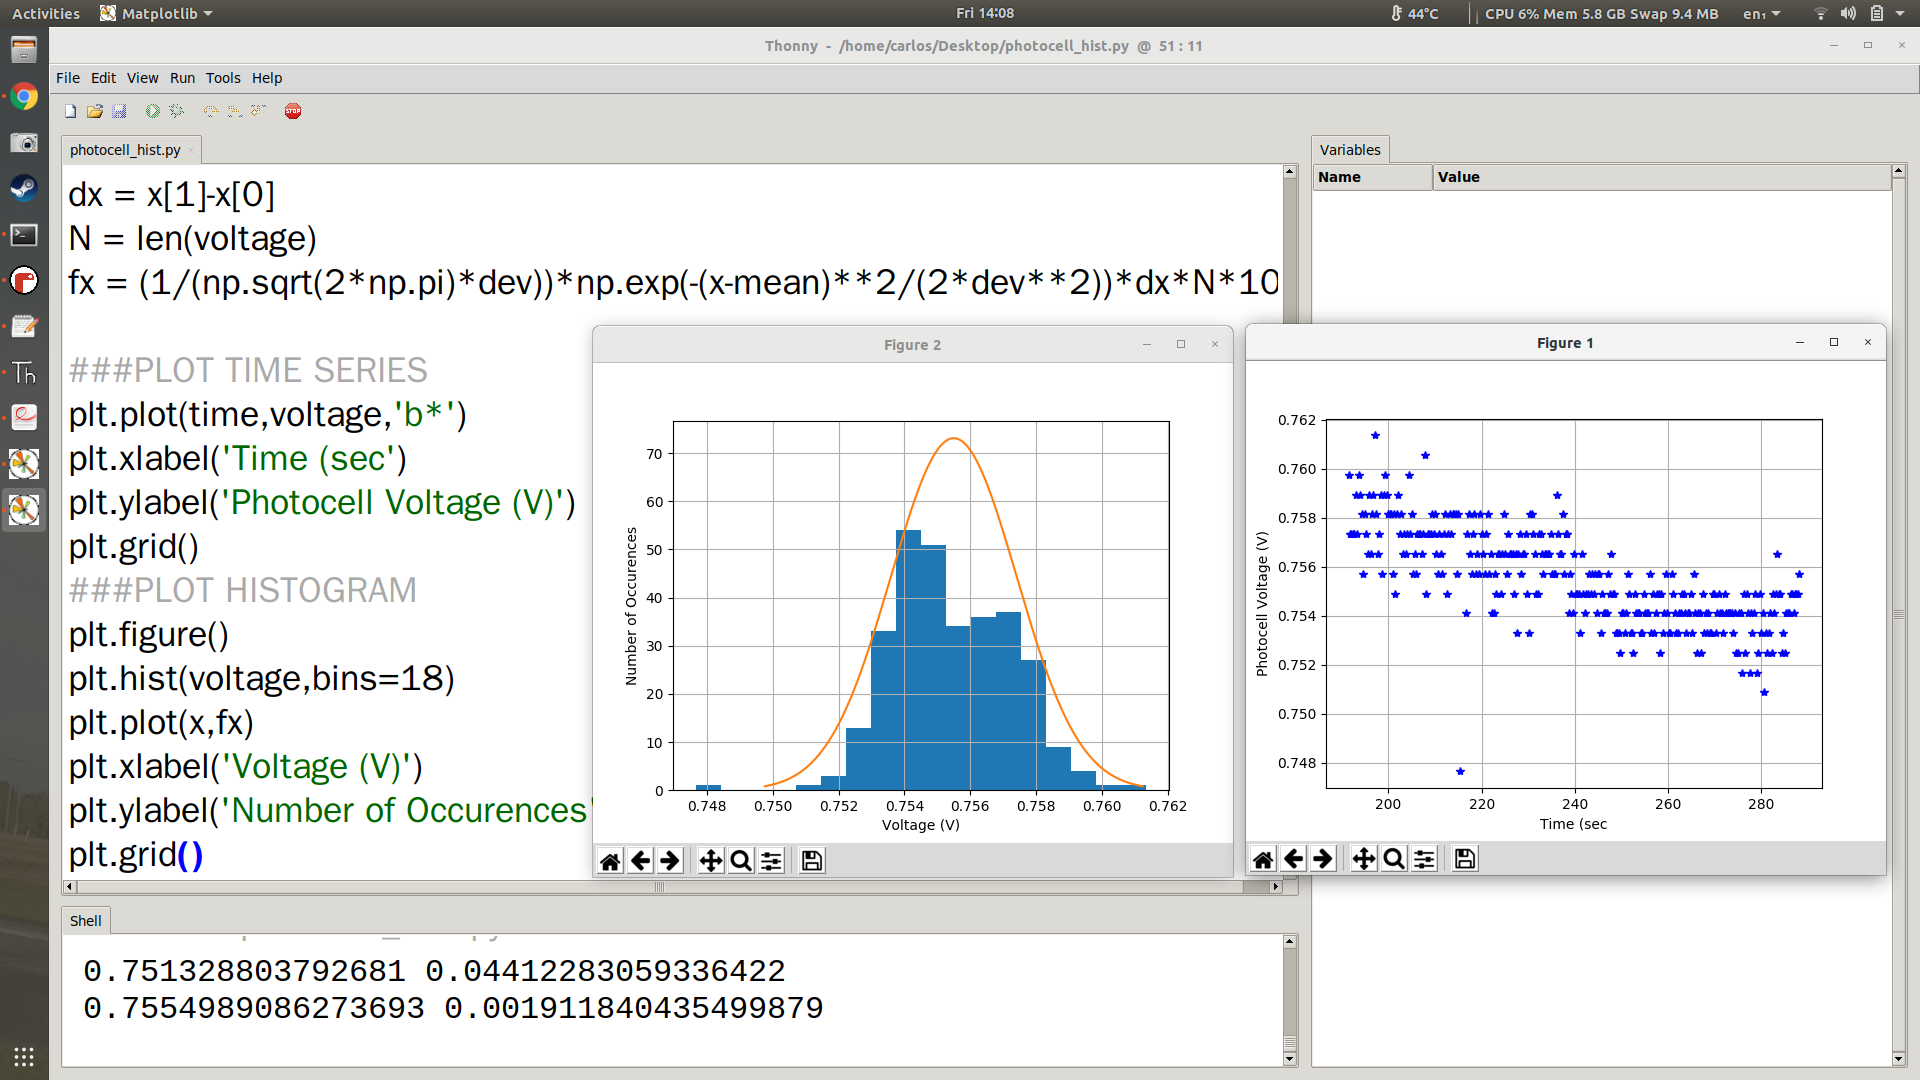
\includegraphics[width=\textwidth]{Figures/histogram_good.png}
  \end{center}
\end{figure}
\subsection{Normal Distribution}
I also was able to plot the Normal Gaussian Distribution on top of the histogram. You can see that in the left plot in orange. The code to do that is shown below where the 72 in the plot is the "height" of the histogram. Note that your histogram will have a different height and you will need to get that specifically from your plot. 
\begin{verbatim}
###COMPUTE THE NORMAL DISTRIBUTION 

x = np.linspace(-3*s+mu,3*s+mu,100) 

pdf = 1.0/(s*np.sqrt(2*np.pi))*np.exp((-(x-mu)**2)/(2.0*s**2)) * (s*np.sqrt(2*np.pi)) * 72
\end{verbatim}
The equations above make a time series from +-3 standard deviations from the mean and then plot the PDF of a normal Gaussian distribution. The only extra thing you have to do is multiply by (s*np.sqrt(2*np.pi)) * 72 which first causes the height of the PDF to be 1 and then multiply by 72 which again is the height of the histogram which will be different for your system.

\subsection{Assignment}

For this assignment you are to build another voltage divider circuit using a photocell and measure the voltage across the photocell using the analog to digital converter on the CPB/CPX. First take 30 seconds of data where you cover the photocell with your hand and also shine a flashlight on it. This will represent the min and max values of Lux as well as the min and max values of the resistance in your photocell. After that you are to run some statistics on the photocell by taking 1000 data points three separate times at three different light levels. The three light levels are low light (hand covered), ambient light (office light or shade light), and high light (flashlight or sunlight). For each set of 1000 data points, create a histogram, compute the mean, median, standard deviation and plot a Gaussian distribution curve on top of the histogram. 

Once you've completed the project above, upload a PDF with all of the photos and text
below included. My recommendation is for you to create a Word document
and insert all the photos and text into the document. Then export the
Word document to a PDF. For videos I suggest uploading the videos to
Google Drive, turn on link sharing and include a link in your
PDF. Note that all code must be included in the appendix or you'll be
penalized 10\%. 

        
\begin{enumerate}[itemsep=-5pt]
\item Include a photo of your circuit and write the value of the resistor that is in series with your photocell. Also, explain how you varied the light levels - 10\%
\item Plot voltage, resistance (converted from voltage) and Lux (converted from resistance) of the photocell vs time for your first 30 seconds of data where you randomly vary light conditions. - 30\%
\item Include the mean, median, and standard deviation of all light levels in Lux - 10\%
\item Include 3 histogram plots of low light, ambient light and high
light levels in units of Lux. On top of the histogram plot the normal Gaussian distribution to see how close your histogram is to a Gaussian distribution - 30\%
\end{enumerate}
